%!TEX root = ../my_thesis.tex
\chapter{Des oscillations du décodage itératif} % (fold)

Dans ce chapitre, on présente le SC et le décodage  à la Benjamin

\vspace*{\fill}
\minitocTITI
\vspace*{\fill}
\newpage

\section{Introduction}\label{sec:ch2_intro} 
En 1996, Benedetto et Montorsi listent les questions ouvertes liées aux turbo codes \cite{benedetto_unveiling}. La
première, qu'ils qualifient de \og question théorique importante \fg concerne la convergence des algorithmes 
sous-optimaux itératifs. \og Convergent-ils toujours ? Sous quelles conditions ? \fg

Peu après, il a été montré par des arguments géométriques que la convergence de ces algorithmes vers la solution à 
maximum de vraisemblance ou vers une solution stable n'est pas garantie \cite{richardson_geometry}.
Dans \cite{reid_convergence}, l'évolution de la valeur des LLR des informations \textit{a posteriori} est présenté au 
cours des itérations. Les auteurs classifient alors le comportement des LLRs lors du décodage des trames selon 3 modes : 
\begin{enumerate}
	\item Tous les bits convergents rapidement et de la même manière vers une solution stable.
	\item La plus part des bits convergent rapidement vers une solution stable alors que les autres convergent de manière 
	différente (croissance plus lente).
	\item Les valeurs des LLR oscillent, croisant ou non le seuil de décision (0). Dans ce cas, l'allure des LLRs est 
	sinusoïdale.
\end{enumerate}
De ces constatations, les auteurs proposent un critère d'arrêt pour le processus itératif basé sur la valeur moyenne des 
LLRs et d'un seuil. Néanmoins, la valeur du seuil ne peut être déterminé que de manière empirique. %Afin d'améliorer les 
%performances 

D'autres critères d'arrêt basés sur l'analyse des changements de signe des informations produites par les décodeur 
élémentaires avaient déjà été proposés dans la littérature. Le Sign Change Ratio (SCR) \cite{fossorier_scr} est une 
approximation du critère basé sur la Cross Entropy (CE) \cite{hagenauer_ce}. Le principe consiste à compter le nombre de 
changement de signes $C(i)$ des information extrinsèques produites par le second SISO entre l'itération $i$ et $i-1$. 
Des simulations montrent qu'arrêter les itérations lorsque $C(i)\leq (0,0005 \sim 0.03)\times K$ permet d'obtenir les 
mêmes performances en termes de nombre d'itérations moyen utilisées et de décodage que le critère CE.

Le critère d'arrêt nommé Sign Difference Ratio (SDR) \cite{fossorier_scr} est une variante du SCR. Dans ce cas, $C(i)$ 
compte le nombre de fois où l'information \textit{a posteriori} et l'information extrinsèque diffèrent à l'itération $i$. 
Ce critère propose les mêmes performances que le SCR tout en permettant de réduire la quantité de stockage nécessaire.

Ainsi, dans le cadre des turbo codes, les oscillations au sein du décodeur ont été étudiées pour mieux comprendre le 
fonctionnement du processus itératif mais aussi pour fournir des critères d'arrêt performants, c'est à dire permettant de 
réduire significativement le nombre d'itération moyen tout en conservant les performances de décodage obtenues avec un 
nombre d'itération fixe maximal.

Dans le cadre des codes LDPC, le processus de décodage est itératif. De même, des phénomènes oscillatoires sont aussi 
observables. Néanmoins dans le cadre des codes LDPC, les équations de parités permettent la détection d'erreurs. Ainsi, 
les oscillations ont été étudiés dans un but d'améliorer des performances de décodage. Deux approches majeures ont été 
considérées. La première approche consiste en une modification de l'algorithme à propagation de croyance (BP) pour le 
décodage des codes LDPC \cite{gounai_bp_osc}. Son principe est le suivant. Si le nouveau LLR extrinsèque (qui correspond 
au calcul des nœuds de variable) change de signe lors de la nouvelle itération, alors la valeur calculée lors de 
l'itération précédente est sommée à la valeur courante. Les auteurs constates des meilleurs performances de décodage en 
comparaison de l'algorithme BP usuel.

La seconde approche, nommée Self-Corrected (SC) \cite{savin_sc}, est une modification de l'algorithme Min-Sum lui même
étant une simplification du BP. Son principe est similaire à l'approche précédente. Si le nouveau LLR extrinsèque change 
de signe lors de la nouvelle itération, alors ce LLR est mis à zéro avant d'être transmis aux nœuds de parités. L'auteur 
présente des gains de performances dans la convergence permettant au SC de gagner 0,4 dB sur le Min-Sum et n'est plus 
qu'à 0,1 dB du BP, bien plus complexe.

Avant de présenter une adaptation de ces approches aux turbo codes, une étude statistique concernant les oscillations 
de l'information extrinsèque au cours du décodage itératif des turbo codes est maintenant mené.

\section{Observations statistiques des oscillations dans le processus de turbo décodage}

\subsection{Cadre de l'étude}
Cette étude se place dans le cadre des turbo codes binaires. Les deux standards considérés sont le standard LTE (8 
états) et le standard CCSDS (16 états). Ces statistiques sont obtenues grâce à un décodeur utilisant l'algorithme 
EML-MAP, itérant jusque 32 fois. Dans un premier temps, des moyennes statistiques sont présentées faisant apparaître une 
corrélation forte entre les oscillations dans la trame et le fait que cette trame soit erronée. Ensuite, ces 
statistiques sont présentées en fonction de l'itération courante. Finalement, les occurrences du nombre d'oscillations
seront présentés suivant qu'un bit soit correct ou non lors de la dernière itération. Toutes ces statistiques sont 
présentées pour plusieurs valeurs de SNR correspondant à des taux d'erreur trame valant $10^{-2}, 10^{-3}, 10^{-4}, 
10^{-5}$.

Au sein d'un turbo décodeur, quatre types d'oscillations des informations extrinsèques peuvent être considérées. Elles 
peuvent survenir en sortie d'un même décodeur élémentaire entre deux itérations. Cela peut correspondre à une 
oscillation du décodeur opérant dans l'ordre naturel (respectivement entrelacé) entre deux itérations, noté alors 
$N\rightarrow N$ (respectivement $I\rightarrow I$). Une oscillation peut aussi se produire entre les deux dimensions. 
Dans ce cas, un des décodeurs à un avis sur un bit et lors de la demi-itération suivante l'autre décodeur a un avis 
opposé. Ces oscilaltions correspondent donc à des désaccord entre les deux décodeurs élémentaires. Ils sont notés 
$N\rightarrow I$ (respectivement $I\rightarrow N$) si la référence est le décodeur opérant dans l'ordre naturel 
(respectivement entrelacé).

La Figure \ref{fig:osc} présente ces 4 types d’oscillations des informations extrinsèques sur un schéma de turbo 
décodeur dans lequel les étapes d'entrelacement n’apparaissent pas pour plus de simplicité.

\begin{figure}[h!]
	\centering
	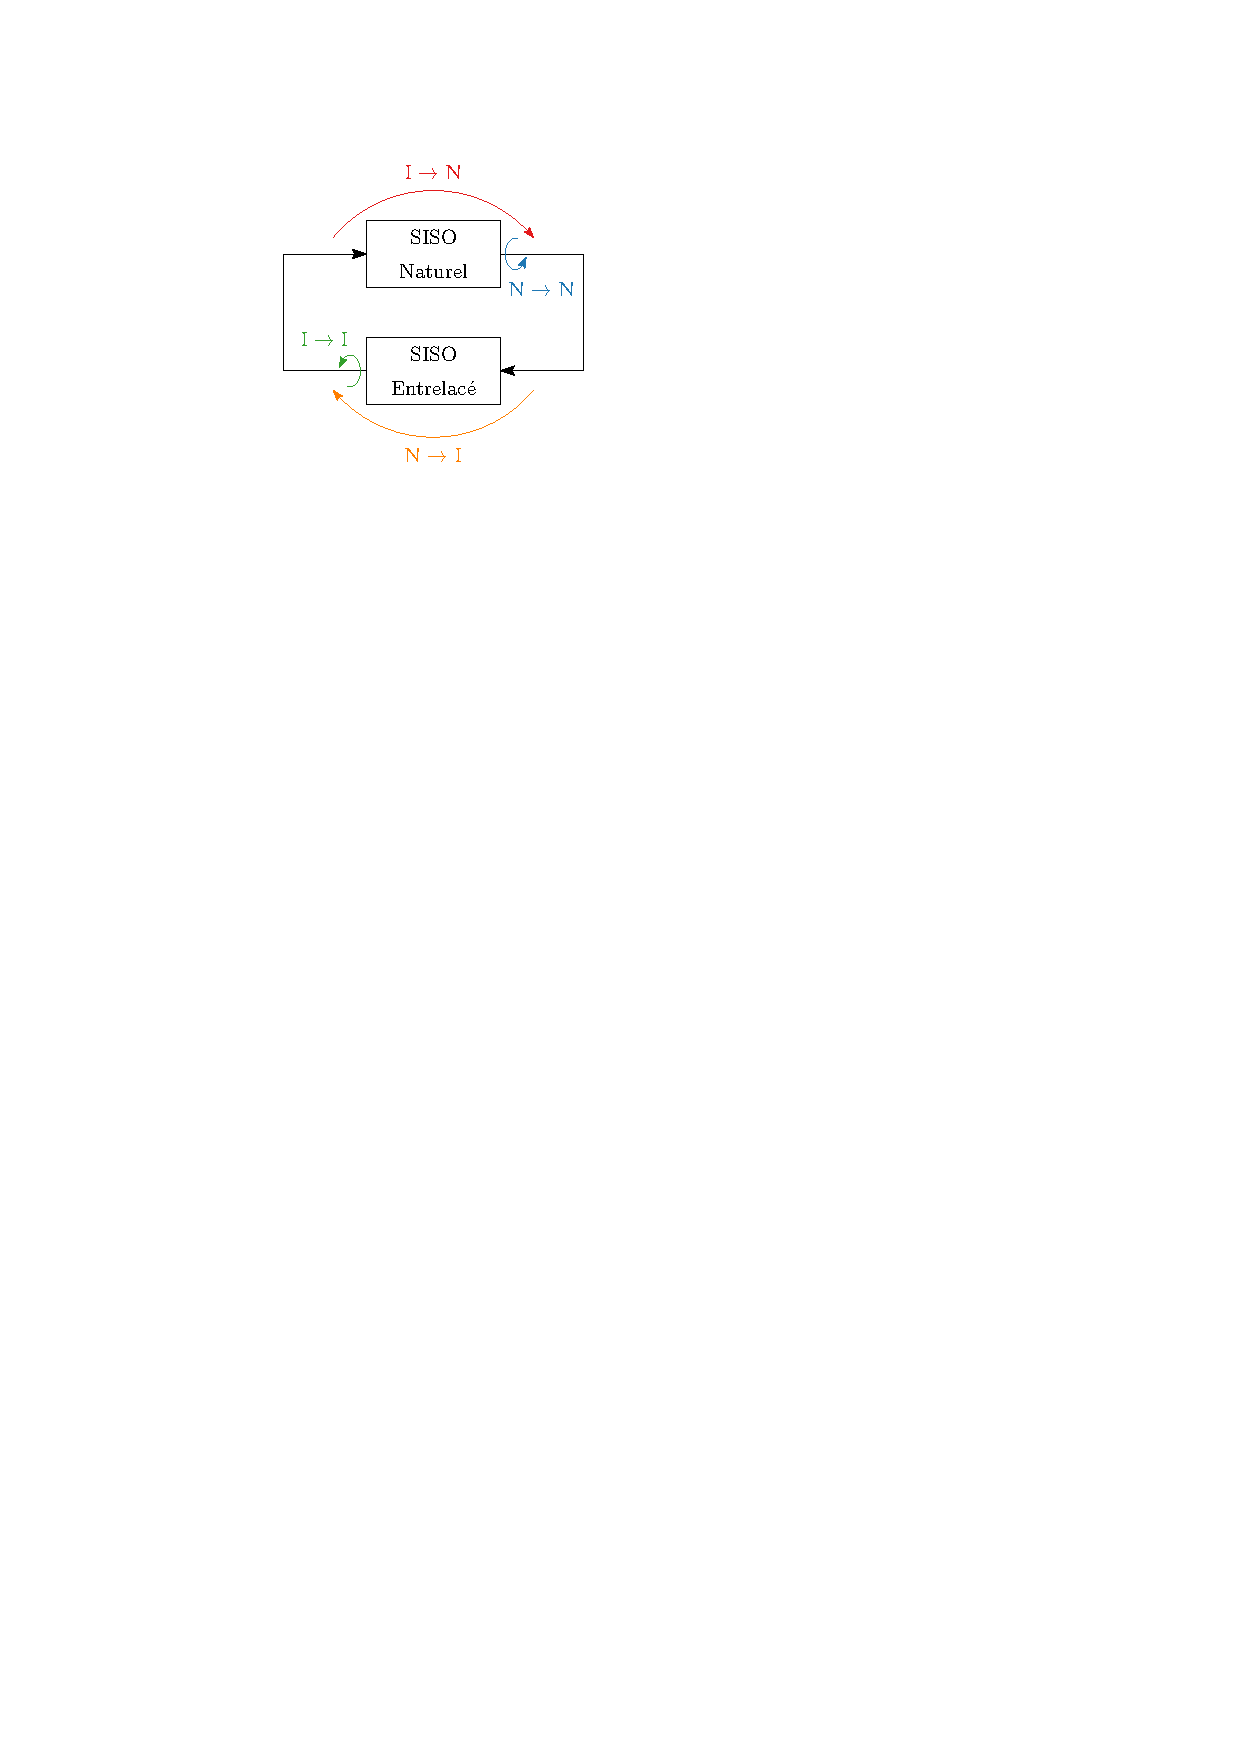
\includegraphics[width=7cm]{main/ch2_fig/ipe/osc.pdf}
	\caption{\label{fig:osc}Les différentes oscillations de l'information extrinsèque possibles.}
\end{figure}

\subsection{Nombre moyen d'oscillations par bit}
Cette section présente 

\begin{figure}[!ht]
	\begin{tikzpicture}
		
		\begin{groupplot}[group style={group name=lte, group size= 2 by 2, horizontal sep=2cm, vertical sep=2cm}, 
					height=0.4\textwidth,  width=0.5\textwidth,
					symbolic x coords={NN, II, NI, IN},
	                xtick=data,
	                %x tick label style= {rotate=45,anchor=north east},
	                ylabel=Nombre d'oscillations par bit,
	                ymin=0, ymax=31,
	                ybar = 1.5pt, /pgf/bar width=8pt,
	                enlarge x limits=0.15, ymajorgrids, grid style={gray!30},legend columns=2]
		\nextgroupplot[legend to name=grouplegend]
                \addplot[fill=falseframe] table [x=X, y=AB] {main/ch2_fig/stats/lte_2/10-2/moyennes.dat}; 
                \addlegendentry{Trames erronées à la dernière itération}
        		\addplot[fill=falsebit] table [x=X, y=EB] {main/ch2_fig/stats/lte_2/10-2/moyennes.dat};  
        		\addlegendentry{Bits erronés dans trames erronées}
        		\addplot[fill=correctbit] table [x=X, y=CB] {main/ch2_fig/stats/lte_2/10-2/moyennes.dat}; 
        		\addlegendentry{Bits justes dans trames erronées} 
        		\addplot[fill=correctframe] table [x=X, y=CF] {main/ch2_fig/stats/lte_2/10-2/moyennes.dat};  
        		\addlegendentry{Trames corrigées à la dernière itération}
        \nextgroupplot[]
	            \addplot[fill=falseframe] table [x=X, y=AB] {main/ch2_fig/stats/lte_2/10-3/moyennes.dat}; 
	    		\addplot[fill=falsebit] table [x=X, y=EB] {main/ch2_fig/stats/lte_2/10-3/moyennes.dat}; 
	    		\addplot[fill=correctbit] table [x=X, y=CB] {main/ch2_fig/stats/lte_2/10-3/moyennes.dat}; 
	    		\addplot[fill=correctframe] table [x=X, y=CF] {main/ch2_fig/stats/lte_2/10-3/moyennes.dat}; 
        \nextgroupplot[]
                \addplot[fill=falseframe] table [x=X, y=AB] {main/ch2_fig/stats/lte_2/10-4/moyennes.dat}; 
        		\addplot[fill=falsebit] table [x=X, y=EB] {main/ch2_fig/stats/lte_2/10-4/moyennes.dat}; 
        		\addplot[fill=correctbit] table [x=X, y=CB] {main/ch2_fig/stats/lte_2/10-4/moyennes.dat}; 
        		\addplot[fill=correctframe] table [x=X, y=CF] {main/ch2_fig/stats/lte_2/10-4/moyennes.dat}; 
        \nextgroupplot[]
                \addplot[fill=falseframe] table [x=X, y=AB] {main/ch2_fig/stats/lte_2/10-5/moyennes.dat}; 
        		\addplot[fill=falsebit] table [x=X, y=EB] {main/ch2_fig/stats/lte_2/10-5/moyennes.dat}; 
        		\addplot[fill=correctbit] table [x=X, y=CB] {main/ch2_fig/stats/lte_2/10-5/moyennes.dat}; 
        		\addplot[fill=correctframe] table [x=X, y=CF] {main/ch2_fig/stats/lte_2/10-5/moyennes.dat}; 
        		\coordinate (bot) at (rel axis cs:1,0);

		\end{groupplot}

		\node[below = 0.8cm of lte c1r1.south] {(a) : FER = $10^{-2}$};
        \node[below = 0.8cm of lte c2r1.south] {(b) : FER = $10^{-3}$};
        \node[below = 0.8cm of lte c1r2.south] {(c) : FER = $10^{-4}$};
        \node[below = 0.8cm of lte c2r2.south] {(d) : FER = $10^{-5}$};

		\node at (lte c1r1.north) [anchor=south, xshift=3.4cm, yshift=1cm] {\ref{grouplegend}};
	\end{tikzpicture}
	\caption{Oscillations moyenne pour différents taux d'erreurs dtrame cibles, standard LTE \label{fig:ltemoy}}
\end{figure}

\begin{figure}[!ht]
	\begin{tikzpicture}
		
		\begin{groupplot}[group style={group name=ccsds, group size= 2 by 2, horizontal sep=2cm, vertical sep=2cm}, 
					height=0.4\textwidth,  width=0.5\textwidth,
					symbolic x coords={NN, II, NI, IN},
	                xtick=data,
	                %x tick label style= {rotate=45,anchor=north east},
	                ylabel=Nombre d'oscillations par bit,
	                ymin=0, ymax=31,
	                ybar = 1.5pt, /pgf/bar width=8pt,
	                enlarge x limits=0.15, ymajorgrids, grid style={gray!30},legend columns=2]
		\nextgroupplot[legend to name=grouplegend]
                \addplot[fill=falseframe] table [x=X, y=AB] {main/ch2_fig/stats/ccsds_2/10-2/moyennes.dat}; 
                \addlegendentry{Trames erronées à la dernière itération}
        		\addplot[fill=falsebit] table [x=X, y=EB] {main/ch2_fig/stats/ccsds_2/10-2/moyennes.dat};  
        		\addlegendentry{Bits erronés dans trames erronées}
        		\addplot[fill=correctbit] table [x=X, y=CB] {main/ch2_fig/stats/ccsds_2/10-2/moyennes.dat}; 
        		\addlegendentry{Bits justes dans trames erronées} 
        		\addplot[fill=correctframe] table [x=X, y=CF] {main/ch2_fig/stats/ccsds_2/10-2/moyennes.dat};  
        		\addlegendentry{Trames corrigées à la dernière itération}
        \nextgroupplot[]
	            \addplot[fill=falseframe] table [x=X, y=AB] {main/ch2_fig/stats/ccsds_2/10-3/moyennes.dat}; 
	    		\addplot[fill=falsebit] table [x=X, y=EB] {main/ch2_fig/stats/ccsds_2/10-3/moyennes.dat}; 
	    		\addplot[fill=correctbit] table [x=X, y=CB] {main/ch2_fig/stats/ccsds_2/10-3/moyennes.dat}; 
	    		\addplot[fill=correctframe] table [x=X, y=CF] {main/ch2_fig/stats/ccsds_2/10-3/moyennes.dat}; 
        \nextgroupplot[]
                \addplot[fill=falseframe] table [x=X, y=AB] {main/ch2_fig/stats/ccsds_2/10-4/moyennes.dat}; 
        		\addplot[fill=falsebit] table [x=X, y=EB] {main/ch2_fig/stats/ccsds_2/10-4/moyennes.dat}; 
        		\addplot[fill=correctbit] table [x=X, y=CB] {main/ch2_fig/stats/ccsds_2/10-4/moyennes.dat}; 
        		\addplot[fill=correctframe] table [x=X, y=CF] {main/ch2_fig/stats/ccsds_2/10-4/moyennes.dat}; 
        \nextgroupplot[]
                \addplot[fill=falseframe] table [x=X, y=AB] {main/ch2_fig/stats/ccsds_2/10-5/moyennes.dat}; 
        		\addplot[fill=falsebit] table [x=X, y=EB] {main/ch2_fig/stats/ccsds_2/10-5/moyennes.dat}; 
        		\addplot[fill=correctbit] table [x=X, y=CB] {main/ch2_fig/stats/ccsds_2/10-5/moyennes.dat}; 
        		\addplot[fill=correctframe] table [x=X, y=CF] {main/ch2_fig/stats/ccsds_2/10-5/moyennes.dat}; 
        		\coordinate (bot) at (rel axis cs:1,0);

		\end{groupplot}

		\node[below = 0.8cm of lte c1r1.south] {(a) : FER = $10^{-2}$};
        \node[below = 0.8cm of lte c2r1.south] {(b) : FER = $10^{-3}$};
        \node[below = 0.8cm of lte c1r2.south] {(c) : FER = $10^{-4}$};
        \node[below = 0.8cm of lte c2r2.south] {(d) : FER = $10^{-5}$};

		\node at (ccsds c1r1.north) [anchor=south, xshift=3.4cm, yshift=1cm] {\ref{grouplegend}};
	\end{tikzpicture}
	\caption{Oscillations moyenne pour différents taux d'erreurs dtrame cibles, standard CCSDS \label{fig:ccsdsmoy}}
\end{figure}